
\section{介质膜问题}

\subsection{光学介质膜}
如图\ref{光学介质膜}，在空气（a端）和基片（g端）之间贴有一张膜，膜由\(N\)层介质堆叠而成.空气的介电常数为\(\varepsilon_a\)，磁导率为\(\mu_a\)，记其特征导纳\(\zeta_a = \sqrt{\varepsilon_a/\mu_a}\).基片的介电常数为\(\varepsilon_g\)，磁导率为\(\mu_g\)，记\(\zeta_g = \sqrt{\varepsilon_g/\mu_g}\).膜的介电常数为\(\varepsilon_m\)，磁导率为\(\mu_m\)，厚度为\(h_m\)，记\(\zeta_m = \sqrt{\varepsilon_m/\mu_m}\).空气、基片、膜在膜平面方向无限延展，可视为一维问题.

现有一束角频率为\(\omega\)的电磁波从空气向基片方向打入，记\(\vb{n}\)为膜平面的法向，\(\vb{\tau}\)方向沿膜平面切向且在入射面内，\(\vb{s}\)方向沿膜平面切向且垂直于入射面，\(\vb{n}-\vb{\tau}-\vb{s}\)构成右手系.定义电磁波的\(\vb{p}\)方向，使得\(\vb{p}-\vb{s}-\vb{k}\)构成右手系，其中\(\vb{k}\)是波矢方向.

入射电磁波（incident ray，简称i）经膜反射回到空气，得到反射电磁波（reflected ray，简称r），或经膜透射至基片内，得到透射电磁波（transmitted ray，简称t）.下研究反射、透射电磁波的能量和偏振状态.

对电磁波引入复相因子\(e^{i(\vb{k}\cdot\vb{r}-\omega t)}\)，记\(\zeta = \sqrt{\varepsilon/\mu}\)，则麦克斯韦方程可简化为：
\begin{equation*}
	\vb{k}\cdot\vb{E} = 0,\quad \vb{k}\cdot\vb{H} = 0,\quad \vb{H} = \zeta\,\vb{k}\times\vb{E},\quad \vb{E} = -\dfrac{1}{\zeta}\,\vb{k}\times\vb{H}.
\end{equation*}

记第\(m\)层介质内的电磁波波矢方向与\(\vb{n}\)夹角为\(\theta_m\)，入射及反射电磁波波矢方向与\(\vb{n}\)夹角为\(\theta_a\)，透射电磁波波矢方向与\(\vb{n}\)夹角为\(\theta_g\)，则
\begin{equation*}
	\sqrt{\varepsilon_m\mu_m}\sin\theta_m = \sqrt{\varepsilon_a\mu_a}\sin\theta_a = \sqrt{\varepsilon_g\mu_g}\sin\theta_g,
\end{equation*}

记第\(m\)层介质上部的\(\vb{s}\)、\(\vb{\tau}\)、\(\vb{p}\)方向总的磁场分量为\(H_s^m\)、\(H_\tau^m\)、\(H_p^m\)，总的电场分量为\(E_s^m\)、\(E_\tau^m\)、\(E_p^m\).a端与第1层介质、第\(N\)层介质与g端用上标a、g表示，入射、反射、透射电磁波用上标i、r、t表示（上标t和g等价，上标a和1等价）.

\(E^m\)和\(H^m\)应当由与入射光同向（\(+\)向）及与反射光同向（\(-\)向）的两类电磁波组成，其振幅记为\(E^{m+}\)、\(E^{m-}\)、\(H^{m+}\)、\(H^{m-}\).易知
\begin{equation*}
	H_\tau^m = (H_p^{m+} - H_p^{m-})\cos\theta_m,\quad E_\tau^m = (E_p^{m+} - E_p^{m-})\cos\theta_m.
\end{equation*}

对于第\(m\)层介质，由切向电场磁场分量连续的边界条件，以及电场磁场的比例关系得：
\begin{equation*}
	E_s^m = E_s^{m+} + E_s^{m-},\quad E_s^{m+1} = e^{i\varphi_m}E_s^{m+} + e^{-i\varphi_m}E_s^{m-},
\end{equation*}
\begin{equation*}
	H_\tau^m = \zeta_m\cos\theta_m(E_s^{m+} - E_s^{m-}),\quad H_\tau^{m+1} = \zeta_m\cos\theta_m(e^{i\varphi_m}E_s^{m+} - e^{-i\varphi_m}E_s^{m-}),
\end{equation*}
\begin{equation*}
	H_s^m = H_s^{m+} + H_s^{m-},\quad H_s^{m+1} = e^{i\varphi_m}H_s^{m+} + e^{-i\varphi_m}H_s^{m-},
\end{equation*}
\begin{equation*}
	E_\tau^m = \zeta_m^{-1}\cos\theta_m(H_s^{m+} - H_s^{m-}),\quad E_\tau^{m+1} = \zeta_m^{-1}\cos\theta_m(e^{i\varphi_m}H_s^{m+} - e^{-i\varphi_m}H_s^{m-}).
\end{equation*}
式中\(\varphi_m\)是电磁波在第\(m\)层介质传播单程的附加相位
\begin{equation*}
	\varphi_m = \omega\sqrt{\varepsilon_m\mu_m}\,h_m\cos\theta_m = \omega h_m\sqrt{\varepsilon_m\mu_m - \varepsilon_a\mu_a\sin^2\theta_a}.
\end{equation*}

由此解得
\begin{equation*}
	\begin{pmatrix}
		E_s^m \\
		H_\tau^m
	\end{pmatrix}
	=
	\begin{pmatrix}
		\cos\varphi_m                      & -i\zeta_m^{-1}\dfrac{\sin\varphi_m}{\cos\theta_m} \\
		-i\zeta_m\cos\theta_m\sin\varphi_m & \cos\varphi_m
	\end{pmatrix}
	\begin{pmatrix}
		E_s^{m+1} \\
		H_\tau^{m+1}
	\end{pmatrix},
\end{equation*}
\begin{equation*}
	\begin{pmatrix}
		H_s^m \\
		E_\tau^m
	\end{pmatrix}
	=
	\begin{pmatrix}
		\cos\varphi_m                           & -i\zeta_m\dfrac{\sin\varphi_m}{\cos\theta_m} \\
		-i\zeta_m^{-1}\cos\theta_m\sin\varphi_m & \cos\varphi_m
	\end{pmatrix}
	\begin{pmatrix}
		H_s^{m+1} \\
		E_\tau^{m+1}
	\end{pmatrix}.
\end{equation*}

因此总的转移矩阵为(运算时可以将\(\zeta\)关于任意标准值无量纲化)：
\begin{equation*}
	P = \prod_{m=1}^{N}
	\begin{pmatrix}
		\cos\varphi_m                      & -i\zeta_m^{-1}\dfrac{\sin\varphi_m}{\cos\theta_m} \\
		-i\zeta_m\cos\theta_m\sin\varphi_m & \cos\varphi_m
	\end{pmatrix}
	=
	\begin{pmatrix}
		P_{11} & P_{12} \\
		P_{21} & P_{22}
	\end{pmatrix},
\end{equation*}
\begin{equation*}
	Q = \prod_{m=1}^{N}
	\begin{pmatrix}
		\cos\varphi_m                           & -i\zeta_m\dfrac{\sin\varphi_m}{\cos\theta_m} \\
		-i\zeta_m^{-1}\cos\theta_m\sin\varphi_m & \cos\varphi_m
	\end{pmatrix}
	=
	\begin{pmatrix}
		Q_{11} & Q_{12} \\
		Q_{21} & Q_{22}
	\end{pmatrix},
\end{equation*}

对应
\begin{equation*}
	\begin{pmatrix}
		E_s^a \\
		H_\tau^a
	\end{pmatrix}
	=
	\begin{pmatrix}
		E_s^1 \\
		H_\tau^1
	\end{pmatrix}
	= P
	\begin{pmatrix}
		E_s^g \\
		H_\tau^g
	\end{pmatrix}
	= P
	\begin{pmatrix}
		E_s^t \\
		H_\tau^t
	\end{pmatrix},
\end{equation*}
\begin{equation*}
	\begin{pmatrix}
		H_s^a \\
		E_\tau^a
	\end{pmatrix}
	=
	\begin{pmatrix}
		H_s^1 \\
		E_\tau^1
	\end{pmatrix}
	= Q
	\begin{pmatrix}
		H_s^g \\
		E_\tau^g
	\end{pmatrix}
	= Q
	\begin{pmatrix}
		H_s^t \\
		E_\tau^t
	\end{pmatrix}.
\end{equation*}

对于a端和g端分析得：
\begin{equation*}
	E_s^a = E_s^i + E_s^r,\quad H_\tau^t = \zeta_g \cos\theta_g E_s^t,\quad H_\tau^a = \zeta_i \cos\theta_a (E_s^i - E_s^r).
\end{equation*}
\begin{equation*}
	H_s^a = \zeta_i (E_p^i + E_p^r),\quad E_\tau^t = \zeta_g \cos\theta_g H_s^t = E_p^t \cos\theta_g,\quad E_\tau^a = \cos\theta_a (E_p^i - E_p^r).
\end{equation*}

联立转移矩阵关系，解得：
\begin{equation*}
	r_s = \dfrac{E_s^r}{E_s^i} = \dfrac{\zeta_a \cos\theta_a (P_{11} + \zeta_g \cos\theta_g P_{12}) - (P_{21} + \zeta_g \cos\theta_g P_{22})}{\zeta_a \cos\theta_a (P_{11} + \zeta_g \cos\theta_g P_{12}) + (P_{21} + \zeta_g \cos\theta_g P_{22})},
\end{equation*}
\begin{equation*}
	t_s = \dfrac{E_s^t}{E_s^i} = \dfrac{2\zeta_a \cos\theta_a}{\zeta_a \cos\theta_a (P_{11} + \zeta_g \cos\theta_g P_{12}) + (P_{21} + \zeta_g \cos\theta_g P_{22})},
\end{equation*}
\begin{equation*}
	r_p = \dfrac{E_p^r}{E_p^i} = \dfrac{\cos\theta_a (Q_{11}\zeta_g + Q_{12}\cos\theta_g) - \zeta_a (Q_{21}\zeta_g + Q_{22}\cos\theta_g)}{\cos\theta_a (Q_{11}\zeta_g + Q_{12}\cos\theta_g) + \zeta_a (Q_{21}\zeta_g + Q_{22}\cos\theta_g)},
\end{equation*}
\begin{equation*}
	t_p = \dfrac{E_p^t}{E_p^i} = \dfrac{2\zeta_a \cos\theta_a}{\cos\theta_a (Q_{11}\zeta_g + Q_{12}\cos\theta_g) + \zeta_a (Q_{21}\zeta_g + Q_{22}\cos\theta_g)}.
\end{equation*}

不难验证，能流密度反射率\(r^2\)、透射率\(\zeta_g t^2/\zeta_a\)总是满足能量守恒方程
\begin{equation*}
	r^2+\dfrac{\zeta_gt^2\cos\theta_g}{\zeta_a \cos\theta_a}=1.
\end{equation*}

观察\(P_m,\,Q_m\)的形式，不难从解析上验证该式的正确性.

\begin{example}
	电磁波正入射，且\(N\)层介质的光学厚度均为电磁波波长的四分之一，即
	\begin{equation*}
		\theta_m = 0,\quad h_m = \dfrac{\pi}{2\omega\sqrt{\varepsilon_m\mu_m}}, \quad \varphi_m = \dfrac{\pi}{2}.
	\end{equation*}

	\begin{equation*}
		P = \prod_{m=1}^{N}
		\begin{pmatrix}
			0         & -i\zeta_m^{-1} \\
			-i\zeta_m & 0
		\end{pmatrix}
		=
		\begin{cases}
			(-1)^{N/2}
			\begin{pmatrix}
				\dfrac{(\zeta_{N})!!}{(\zeta_{N-1})!!} & 0                                      \\[8pt]
				0                                      & \dfrac{(\zeta_{N-1})!!}{(\zeta_{N})!!}
			\end{pmatrix}, & N\,\text{even}. \\[20pt]
			i(-1)^{(N+1)/2}
			\begin{pmatrix}
				0                                      & \dfrac{(\zeta_{N-1})!!}{(\zeta_{N})!!} \\[8pt]
				\dfrac{(\zeta_{N})!!}{(\zeta_{N-1})!!} & 0
			\end{pmatrix}, & N\,\text{odd}
		\end{cases}
	\end{equation*}

	\begin{equation*}
		Q = \prod_{m=1}^{N}
		\begin{pmatrix}
			0              & -i\zeta_m \\
			-i\zeta_m^{-1} & 0
		\end{pmatrix}
		=
		\begin{cases}
			(-1)^{N/2}
			\begin{pmatrix}
				\dfrac{(\zeta_{N-1})!!}{(\zeta_{N})!!} & 0                                      \\[8pt]
				0                                      & \dfrac{(\zeta_{N})!!}{(\zeta_{N-1})!!}
			\end{pmatrix}, & N\,\text{even}. \\[20pt]
			i(-1)^{(N-1)/2}
			\begin{pmatrix}
				0                                      & \dfrac{(\zeta_{N})!!}{(\zeta_{N-1})!!} \\[8pt]
				\dfrac{(\zeta_{N-1})!!}{(\zeta_{N})!!} & 0
			\end{pmatrix}, & N\,\text{odd}
		\end{cases}
	\end{equation*}

	\begin{equation*}
		r_s = -r_p =
		\begin{cases}
			\dfrac{\zeta_a - \zeta_g \left(\dfrac{(\zeta_{N-1})!!}{(\zeta_{N})!!}\right)^2}{\zeta_a + \zeta_g \left(\dfrac{(\zeta_{N-1})!!}{(\zeta_{N})!!}\right)^2}, & N\,\text{even}. \\[24pt]
			\dfrac{\zeta_a\zeta_g - \left(\dfrac{(\zeta_{N})!!}{(\zeta_{N-1})!!}\right)^2}{\zeta_a\zeta_g + \left(\dfrac{(\zeta_{N})!!}{(\zeta_{N-1})!!}\right)^2},   & N\,\text{odd}
		\end{cases}\quad
		t_s = t_p =
		\begin{cases}
			\dfrac{2(-1)^{N/2}\zeta_a}{\zeta_a \dfrac{(\zeta_{N})!!}{(\zeta_{N-1})!!} + \zeta_g \dfrac{(\zeta_{N-1})!!}{(\zeta_{N})!!}},         & N\,\text{even}. \\[24pt]
			\dfrac{2    i(-1)^{(N-1)/2}\zeta_a}{\dfrac{(\zeta_{N})!!}{(\zeta_{N-1})!!} + \zeta_a\zeta_g \dfrac{(\zeta_{N-1})!!}{(\zeta_{N})!!}}, & N\,\text{odd}
		\end{cases}
	\end{equation*}

	其中\((\zeta_{N})!! =
	\begin{cases}
		\zeta_{N}\zeta_{N-2}\cdots\zeta_2, & N\,\text{even}. \\
		\zeta_{N}\zeta_{N-2}\cdots\zeta_1, & N\,\text{odd}
	\end{cases}\)
\end{example}

\begin{example}
	不存在膜，即\(N = 0\), \(P = Q =
	\begin{pmatrix}
		1 & 0 \\
		0 & 1
	\end{pmatrix}\).
	\begin{equation*}
		r_s = \dfrac{\zeta_a \cos\theta_a - \zeta_g \cos\theta_g}{\zeta_a \cos\theta_a + \zeta_g \cos\theta_g},\quad t_s = \dfrac{2\zeta_a \cos\theta_a}{\zeta_a \cos\theta_a + \zeta_g \cos\theta_g}.
	\end{equation*}
	\begin{equation*}
		r_p = \dfrac{\zeta_g \cos\theta_a - \zeta_a \cos\theta_g}{\zeta_a \cos\theta_g + \zeta_g \cos\theta_a},\quad t_p = \dfrac{2\zeta_a \cos\theta_a}{\zeta_a \cos\theta_g + \zeta_g \cos\theta_a}.
	\end{equation*}
	对应我们熟悉的菲涅尔公式.
\end{example}

\begin{example}
	存在一层膜，即\(N = 1\),
	\begin{equation*}
		P =
		\begin{pmatrix}
			\cos\varphi_1                        & -i\zeta_1^{-1}\dfrac{\sin\varphi_1}{\cos\theta_1} \\
			-i\zeta_1 \cos\theta_1 \sin\varphi_1 & \cos\varphi_1
		\end{pmatrix},\quad
		Q =
		\begin{pmatrix}
			\cos\varphi_1                             & -i\zeta_1\dfrac{\sin\varphi_1}{\cos\theta_1} \\
			-i\zeta_1^{-1} \cos\theta_1 \sin\varphi_1 & \cos\varphi_1
		\end{pmatrix}.
	\end{equation*}
	\begin{equation*}
		r_s = \dfrac{(\zeta_a \cos\theta_a - \zeta_g \cos\theta_g)\cos\theta_1 \cos\varphi_1 - i(-\zeta_1 \cos^2\theta_1 + \zeta_a\zeta_g\zeta_1^{-1}\cos\theta_a\cos\theta_g)\sin\varphi_1}{(\zeta_a \cos\theta_a + \zeta_g \cos\theta_g)\cos\theta_1 \cos\varphi_1 - i(\zeta_1 \cos^2\theta_1 + \zeta_a\zeta_g\zeta_1^{-1}\cos\theta_a\cos\theta_g)\sin\varphi_1},
	\end{equation*}
	\begin{equation*}
		t_s = \dfrac{2\zeta_a \cos\theta_a \cos\theta_1}{(\zeta_a \cos\theta_a + \zeta_g \cos\theta_g)\cos\theta_1 \cos\varphi_1 - i(\zeta_1 \cos^2\theta_1 + \zeta_a\zeta_g\zeta_1^{-1}\cos\theta_a\cos\theta_g)\sin\varphi_1},
	\end{equation*}
	\begin{equation*}
		r_p = \dfrac{(\zeta_g \cos\theta_a - \zeta_a \cos\theta_g)\cos\theta_1 \cos\varphi_1 - i(\zeta_1 \cos\theta_a\cos\theta_g - \zeta_a\zeta_g\zeta_1^{-1}\cos^2\theta_1)\sin\varphi_1}{(\zeta_g \cos\theta_a + \zeta_a \cos\theta_g)\cos\theta_1 \cos\varphi_1 - i(\zeta_1 \cos\theta_a\cos\theta_g + \zeta_a\zeta_g\zeta_1^{-1}\cos^2\theta_1)\sin\varphi_1},
	\end{equation*}
	\begin{equation*}
		t_p = \dfrac{2\zeta_a \cos\theta_a \cos\theta_1}{(\zeta_g \cos\theta_a + \zeta_a \cos\theta_g)\cos\theta_1 \cos\varphi_1 - i(\zeta_1 \cos\theta_a\cos\theta_g + \zeta_a\zeta_g\zeta_1^{-1}\cos^2\theta_1)\sin\varphi_1}.
	\end{equation*}
	对应我们熟悉的FP腔.
\end{example}

\subsection{弹性介质膜}
\subsubsection{弹性介质基本性质}

均匀各项同性的线性弹性介质中，应力张量 \(\vb{T}\) 与位移矢量 \(\vb{u}\) 的关系为
\begin{equation*}
	\vb{T} = \lambda (\nabla \cdot \vb{u}) \vb{I} + \mu \left( (\nabla \vb{u})^\top + \nabla \vb{u} \right).
\end{equation*}
其中 \(\lambda, \mu\) 为Lame系数，与杨氏模量\(E\)和泊松比\(\nu\)的转换关系为
\begin{equation*}
	\lambda = \dfrac{E\nu}{(1 + \nu)(1 - 2\nu)}, \quad \mu = \dfrac{E}{2(1 + \nu)}.
\end{equation*}

记介质质量密度为\(\rho\)，则质元在弹性力作用下的运动方程为
\begin{equation*}
	\rho \dfrac{\partial^2 \vb{u}}{\partial t^2} = \nabla \cdot \vb{T} = (\mu + \lambda) \nabla (\nabla \cdot \vb{u}) + \mu \nabla^2 \vb{u}.
\end{equation*}

对位移矢量做Helmholtz分解，\(\vb{u} = \nabla \phi + \nabla \times \vb{\psi}\)，并取规范 \(\nabla \cdot \vb{\psi} = 0\)，回代运动方程得
\begin{equation*}
	\rho \dfrac{\partial^2 \phi}{\partial t^2} = (\lambda + 2\mu) \nabla^2 \phi, \quad \rho \dfrac{\partial^2 \vb{\psi}}{\partial t^2} = \mu \nabla^2 \vb{\psi}.
\end{equation*}

这说明，介质中存在两种速率的波，纵波 (P波) \(\phi\)和横波 (S波) \(\vb{\psi}\)，其波动形式解为
\begin{equation*}
	\phi \propto e^{i(\vb{k}_P \cdot \vb{r} - \omega t)}, \quad c_P = \dfrac{\omega}{k_P} = \sqrt{\dfrac{\lambda + 2\mu}{\rho}}.\qquad{\psi} \propto e^{i(\vb{k}_S \cdot \vb{r} - \omega t)}, \quad c_S = \dfrac{\omega}{k_S} = \sqrt{\dfrac{\mu}{\rho}}.
\end{equation*}

在弹性波的作用下，位移矢量和应力张量可简化为
\begin{equation*}
	\vb{u} = i \left( \vb{k}_P \phi + \vb{k}_S \times \vb{\psi} \right),
\end{equation*}
\begin{equation*}
	\vb{T} = -\left( \lambda k_P^2 \phi \vb{I} + 2\mu \vb{k}_P \vb{k}_P \phi + \mu (\vb{k}_S \times \vb{\psi}) \vb{k}_S + \mu \vb{k}_S (\vb{k}_S \times \vb{\psi}) \right).
\end{equation*}

在介质交界处，记边界的外法向量为 \(\uv{z}\)，传播方向与法向的夹角均用 \(\theta\)表示，选取 \(x\text{-}z\) 为入射面、\(x\text{-}y\text{-}z\)构成右手系.在焊接良好的理想边界上，位移矢量 \(\vb{u}\) 和法向力 \(\vb{T} \cdot \uv{z}\) 连续.

由于波速不同，入射的P波和S波可以分开考虑、独立叠加，而分析 \(\vb{u}, \vb{T}\) 的形式易知，S波中 \(\vb{\psi}\) 垂直于入射面的部分 (SV波) 和平行于入射面的部分 (SH波) 对边界条件互不干扰，因此入射波的三类偏振情况完全可以分开考虑.再分析边界条件知，只入射P波或SV波时，反射、透射波通常既有P波也有SV波；而只入射SH波时，反射、透射波只有SH波.

\subsubsection{平面弹性介质膜}

具体考虑如图\ref{弹性介质膜}的介质膜.在入射端\(a\)和出射端\(g\)之间有\(N\)层无穷大平板介质膜，第\(m\)层介质的Lame系数为\(\lambda_m, \mu_m\)，厚度为\(h_m\)，质量密度为 \(\rho_s \eta_m\)（\(\rho_s\)是用于无量纲化的标准质量密度），\(a\)和\(g\)介质的Lame系数为\(\lambda_a, \mu_a\)和\(\lambda_g, \mu_g\)，质量密度为 \(\rho_s \eta_a, \rho_s \eta_g\)，各介质的 \(k, c_S, c_P\) 参量定义同上，角频率为 \(\omega\)的弹性波从\(a\)端入射.

易见，切向波矢连续的条件贯穿始终，对任意介质，总有
\begin{equation*}
	k_x = k_P \sin\theta_P = k_S \sin\theta_S.
\end{equation*}

也即
\begin{equation*}
	\sqrt{\dfrac{\eta_a}{\lambda_a + 2\mu_a}} \sin\theta_{Pa} = \sqrt{\dfrac{\eta_a}{\mu_a}} \sin\theta_{Sa} = \sqrt{\dfrac{\eta_m}{\lambda_m + 2\mu_m}} \sin\theta_{Pm} = \sqrt{\dfrac{\eta_m}{\mu_m}} \sin\theta_{Sm} = \sqrt{\dfrac{\eta_g}{\lambda_g + 2\mu_g}} \sin\theta_{Pg} = \sqrt{\dfrac{\eta_g}{\mu_g}} \sin\theta_{Sg}.
\end{equation*}

记弹性波在第\(m\)层介质传播时的相位差为
\begin{equation*}
	\varphi_{Pm} = k_{Pm} h_m \cos\theta_{Pm}, \quad \varphi_{Sm} = k_{Sm} h_m \cos\theta_{Sm}.
\end{equation*}

【只入射P波或SV波】

此时 \(\vb{\psi} = \psi \uv{y}\), \(u_y = 0, T_{yz} = 0\)，边界上的位移和应力为
\begin{equation*}
	u_x &= i \left( k_x \phi - k_{zS} \psi \right) = i k_x \left( \phi \mp \cot\theta_S \psi \right)\\
	u_z &= i \left( k_{zP} \phi + k_x \psi \right) = i k_x \left( \pm \cot\theta_P \phi + \psi \right)\\
	T_{xz} &= -\left( 2\mu k_x k_{zP} \phi + \mu (k_x^2 - k_{zS}^2) \psi \right) = -\rho_s \eta \omega^2 \left( \pm \kappa \sin2\theta_P \phi - \cos2\theta_S \psi \right)\\
	T_{zz} &= -\left( \lambda k_P^2 \phi + 2\mu k_{zP}^2 \phi + 2\mu k_x k_{zS} \psi \right) = -\rho_s \eta \omega^2 \left( \cos2\theta_S \phi \pm \sin2\theta_S \psi \right).
\end{equation*}
其中，沿 \(\pm \uv{z}\) 传播分别取上/下符号，\(\kappa\) 定义为
\begin{equation*}
	\kappa = \dfrac{k_P^2}{k_S^2} = \dfrac{c_S^2}{c_P^2} = \dfrac{\mu}{\lambda + 2\mu}.
\end{equation*}

省去不必要的常数，令 \(\tilde{u}_x = u_x/i k_x\), \(\tilde{u}_z = u_z/i k_x\), \(\tilde{T}_{xz} = -T_{xz}/\rho_s \omega^2\), \(\tilde{T}_{zz} = -T_{zz}/\rho_s \omega^2\).记沿 \(\pm \uv{z}\) 传播的位移标势/矢势为 \(\phi^\pm, \psi^\pm\)，得
\begin{equation*}
	\begin{pmatrix} \tilde{u}_x \\ \tilde{u}_z \\ \tilde{T}_{xz} \\ \tilde{T}_{zz} \end{pmatrix} =
	\begin{pmatrix}
		1                         & 1                          & -\cot\theta_S       & \cot\theta_S        \\
		\cot\theta_P              & -\cot\theta_P              & 1                   & 1                   \\
		\eta \kappa \sin2\theta_P & -\eta \kappa \sin2\theta_P & -\eta \cos2\theta_S & -\eta \cos2\theta_S \\
		\eta \cos2\theta_S        & \eta \cos2\theta_S         & \eta \sin2\theta_S  & -\eta \sin2\theta_S
	\end{pmatrix}
	\begin{pmatrix} \phi^+ \\ \phi^- \\ \psi^+ \\ \psi^- \end{pmatrix}.
\end{equation*}

故第\(m\)层上方与第\(m + 1\) 层上方的位移、应力满足线性关系式
\begin{equation*}
	&\left( \tilde{u}_x^m,\; \tilde{u}_z^m,\; \tilde{T}_{xz}^m,\; \tilde{T}_{zz}^m \right)^\top = P_m \left( \tilde{u}_x^{m+1},\; \tilde{u}_z^{m+1},\; \tilde{T}_{xz}^{m+1},\; \tilde{T}_{zz}^{m+1} \right)^\top.\\
	&P_m = \begin{pmatrix}
		1                                & 1                                 & -\cot\theta_{Sm}         & \cot\theta_{Sm}          \\
		\cot\theta_{Pm}                  & -\cot\theta_{Pm}                  & 1                        & 1                        \\
		\eta_m \kappa_m \sin2\theta_{Pm} & -\eta_m \kappa_m \sin2\theta_{Pm} & -\eta_m \cos2\theta_{Sm} & -\eta_m \cos2\theta_{Sm} \\
		\eta_m \cos2\theta_{Sm}          & \eta_m \cos2\theta_{Sm}           & \eta_m \sin2\theta_{Sm}  & -\eta_m \sin2\theta_{Sm}
	\end{pmatrix} \\
	&\qquad \cdot \begin{pmatrix}
		e^{i\varphi_{Pm}}                                  & e^{-i\varphi_{Pm}}                                   & -\cot\theta_{Sm} e^{i\varphi_{Sm}}         & \cot\theta_{Sm} e^{-i\varphi_{Sm}}          \\
		\cot\theta_{Pm} e^{i\varphi_{Pm}}                  & -\cot\theta_{Pm} e^{-i\varphi_{Pm}}                  & e^{i\varphi_{Sm}}                          & e^{-i\varphi_{Sm}}                          \\
		\eta_m \kappa_m \sin2\theta_{Pm} e^{i\varphi_{Pm}} & -\eta_m \kappa_m \sin2\theta_{Pm} e^{-i\varphi_{Pm}} & -\eta_m \cos2\theta_{Sm} e^{i\varphi_{Sm}} & -\eta_m \cos2\theta_{Sm} e^{-i\varphi_{Sm}} \\
		\eta_m \cos2\theta_{Sm} e^{i\varphi_{Pm}}          & \eta_m \cos2\theta_{Sm} e^{-i\varphi_{Pm}}           & \eta_m \sin2\theta_{Sm} e^{i\varphi_{Sm}}  & -\eta_m \sin2\theta_{Sm} e^{-i\varphi_{Sm}}
	\end{pmatrix}^{-1}.
\end{equation*}

\(P_m\) 四个列向量的解析式如下
\begin{align*}
	P_m|_1 & =
	\begin{pmatrix}
		\cos2\theta_{Sm} \cos\varphi_{Sm} + 2\cos\varphi_{Pm} \sin^2\theta_{Sm}                                                                      \\
		-i \left( 2\cot\theta_{Pm} \sin^2\theta_{Sm} \sin\varphi_{Pm} - \sin\varphi_{Sm} \tan\theta_{Sm} \cos2\theta_{Sm} \right)                    \\
		-i \eta_m \left( 2\sin2\theta_{Pm} \sin^2\theta_{Sm} \sin\varphi_{Pm} \kappa_m + \cos^22\theta_{Sm} \sin\varphi_{Sm} \tan\theta_{Sm} \right) \\
		2\eta_m \cos2\theta_{Sm} \sin^2\theta_{Sm} \left( \cos\varphi_{Pm} - \cos\varphi_{Sm} \right)
	\end{pmatrix}
	\\[2ex]
	P_m|_2 & =
	\begin{pmatrix}
		\dfrac{i \left( -\cos2\theta_{Sm} \sin\varphi_{Pm} + \cot\theta_{Sm} \sin2\theta_{Pm} \sin\varphi_{Sm} \kappa_m \right)}{\cos2\theta_{Sm} \cot\theta_{Pm} + \sin2\theta_{Pm} \kappa_m} \\
		\dfrac{\cos2\theta_{Sm} \cos\varphi_{Pm} \cot\theta_{Pm} + \cos\varphi_{Sm} \sin2\theta_{Pm} \kappa_m}{\cos2\theta_{Sm} \cot\theta_{Pm} + \sin2\theta_{Pm} \kappa_m}                   \\
		\dfrac{2\eta_m \kappa_m \left( \cos\varphi_{Pm} - \cos\varphi_{Sm} \right)}{\csc^2\theta_{Pm} + 2\sec2\theta_{Sm} \kappa_m}                                                            \\
		\dfrac{-i \eta_m \left( \cos^22\theta_{Sm} \sin\varphi_{Pm} + \sin2\theta_{Pm} \sin2\theta_{Sm} \sin\varphi_{Sm} \kappa_m \right)}{\cos2\theta_{Sm} \cot\theta_{Pm} + \sin2\theta_{Pm} \kappa_m}
	\end{pmatrix}
	\\[2ex]
	P_m|_3 & =
	\begin{pmatrix}
		\dfrac{-i \left( \sin\varphi_{Pm} + \cot\theta_{Pm} \cot\theta_{Sm} \sin\varphi_{Sm} \right)}{\left( \cos2\theta_{Sm} \cot\theta_{Pm} + \sin2\theta_{Pm} \kappa_m \right) \eta_m} \\
		\dfrac{\left( \cos\varphi_{Pm} - \cos\varphi_{Sm} \right) \cot\theta_{Pm}}{\left( \cos2\theta_{Sm} \cot\theta_{Pm} + \sin2\theta_{Pm} \kappa_m \right) \eta_m}                    \\
		\dfrac{\cos2\theta_{Sm} \cos\varphi_{Sm} \cot\theta_{Pm} + \cos\varphi_{Pm} \sin2\theta_{Pm} \kappa_m}{\cos2\theta_{Sm} \cot\theta_{Pm} + \sin2\theta_{Pm} \kappa_m}              \\
		\dfrac{-i \left( \cos2\theta_{Sm} \sin\varphi_{Pm} - \cot\theta_{Pm} \sin2\theta_{Sm} \sin\varphi_{Sm} \right)}{\cos2\theta_{Sm} \cot\theta_{Pm} + \sin2\theta_{Pm} \kappa_m}
	\end{pmatrix}
	\\[2ex]
	P_m|_4 & =
	\begin{pmatrix}
		\dfrac{\cos\varphi_{Pm} - \cos\varphi_{Sm}}{\eta_m}                                                              \\
		\dfrac{-i \left( \cot\theta_{Pm} \sin\varphi_{Pm} + \sin\varphi_{Sm} \tan\theta_{Sm} \right)}{\eta_m}            \\
		-i \left( \sin2\theta_{Pm} \sin\varphi_{Pm} \kappa_m - \cos2\theta_{Sm} \sin\varphi_{Sm} \tan\theta_{Sm} \right) \\
		\cos2\theta_{Sm} \cos\varphi_{Pm} + 2\cos\varphi_{Sm} \sin^2\theta_{Sm}
	\end{pmatrix}.
\end{align*}



进而，入射端与出射端的位移、应力满足线性变换\(P = \prod_{m=1}^N P_m, \quad
\left( \tilde{u}_x^a, \tilde{u}_z^a, \tilde{T}_{xz}^a, \tilde{T}_{zz}^a \right)^\top = P \left( \tilde{u}_x^g, \tilde{u}_z^g, \tilde{T}_{xz}^g, \tilde{T}_{zz}^g \right)^\top.\)

代入具体的入射 (i)、反射 (r)、透射 (t) 的标势、矢势
\begin{equation*}
	\tilde{u}_x^a = (\phi_i + \phi_r) - \cot\theta_{Sa} (\psi_i - \psi_r), \quad \tilde{u}_x^g = \phi_t - \cot\theta_{Sg} \psi_t.
\end{equation*}
\begin{equation*}
	\tilde{u}_z^a = \cot\theta_{Pa} (\phi_i - \phi_r) + (\psi_i + \psi_r), \quad \tilde{u}_z^g = \cot\theta_{Pg} \phi_t + \psi_t.
\end{equation*}
\begin{equation*}
	\tilde{T}_{xz}^a = \eta_a \kappa_a \sin2\theta_{Pa} (\phi_i - \phi_r) - \eta_a \cos2\theta_{Sa} (\psi_i + \psi_r), \quad \tilde{T}_{xz}^g = \eta_g \kappa_g \sin2\theta_{Pg} \phi_t - \eta_g \cos2\theta_{Sg} \psi_t.
\end{equation*}
\begin{equation*}
	\tilde{T}_{zz}^a = \eta_a \cos2\theta_{Sa} (\phi_i + \phi_r) + \eta_a \sin2\theta_{Sa} (\psi_i - \psi_r), \quad \tilde{T}_{zz}^g = \eta_g \cos2\theta_{Sg} \phi_t + \eta_g \sin2\theta_{Sg} \psi_t.
\end{equation*}
得到可以解出 \(\phi_r, \psi_r, \phi_t, \psi_t\) 的方程组
\begin{equation*}
	&\begin{pmatrix} -1 \\ \cot\theta_{Pa} \\ \eta_a \kappa_a \sin2\theta_{Pa} \\ -\eta_a \cos2\theta_{Sa} \end{pmatrix} \phi_r +
	\begin{pmatrix} -\cot\theta_{Sa} \\ -1 \\ \eta_a \cos2\theta_{Sa} \\ \eta_a \sin2\theta_{Sa} \end{pmatrix} \psi_r +
	P \begin{pmatrix} 1 \\ \cot\theta_{Pg} \\ \eta_g \kappa_g \sin2\theta_{Pg} \\ \eta_g \cos2\theta_{Sg} \end{pmatrix} \phi_t +
	P \begin{pmatrix} -\cot\theta_{Sg} \\ 1 \\ -\eta_g \cos2\theta_{Sg} \\ \eta_g \sin2\theta_{Sg} \end{pmatrix} \psi_t \\&\qquad=
	\begin{pmatrix} 1 \\ \cot\theta_{Pa} \\ \eta_a \kappa_a \sin2\theta_{Pa} \\ \eta_a \cos2\theta_{Sa} \end{pmatrix} \phi_i +
	\begin{pmatrix} -\cot\theta_{Sa} \\ 1 \\ -\eta_a \cos2\theta_{Sa} \\ \eta_a \sin2\theta_{Sa} \end{pmatrix} \psi_i.
\end{equation*}

对于P波入射，\(\psi_i = 0\)；对于SV波入射，\(\phi_i = 0\)，可解出对应的反射、透射势.

从能量守恒的角度，可以验证以上结果的正确性.波的法向能流密度为
\begin{equation*}
	S_{zP} = \dfrac{1}{2} \rho c_P k_P^2 |\phi|^2 \cos\theta_P = \dfrac{1}{2} \rho_s \omega^2 \dfrac{\eta |\phi|^2}{c_P} \cos\theta_P, \quad S_{zS} = \dfrac{1}{2} \rho_s \omega^2 \dfrac{\eta |\vb{\psi}|^2}{c_S} \cos\theta_S.
\end{equation*}

因此P波入射的解总满足
\begin{equation*}
	\left| \dfrac{\phi_r}{\phi_i} \right|^2 + \dfrac{c_{Pa} \cos\theta_{Sa}}{c_{Sa} \cos\theta_{Pa}} \left| \dfrac{\psi_r}{\phi_i} \right|^2 + \dfrac{\eta_g c_{Pa} \cos\theta_{Pg}}{\eta_a c_{Pg} \cos\theta_{Pa}} \left| \dfrac{\phi_t}{\phi_i} \right|^2 + \dfrac{\eta_g c_{Pa} \cos\theta_{Sg}}{\eta_a c_{Sg} \cos\theta_{Pa}} \left| \dfrac{\psi_t}{\phi_i} \right|^2 = 1.
\end{equation*}

SV入射的解总满足
\begin{equation*}
	\left| \dfrac{\psi_r}{\psi_i} \right|^2 + \dfrac{c_{Sa} \cos\theta_{Pa}}{c_{Pa} \cos\theta_{Sa}} \left| \dfrac{\phi_r}{\psi_i} \right|^2 + \dfrac{\eta_g c_{Sa} \cos\theta_{Sg}}{\eta_a c_{Sg} \cos\theta_{Sa}} \left| \dfrac{\psi_t}{\psi_i} \right|^2 + \dfrac{\eta_g c_{Sa} \cos\theta_{Pg}}{\eta_a c_{Pg} \cos\theta_{Sa}} \left| \dfrac{\phi_t}{\psi_i} \right|^2 = 1.
\end{equation*}


【只入射SH波】

此时 \(\phi = 0\)，\(\vb{k}_S \times \vb{\psi} = k_S \psi \uv{y}\)，边界上的位移和应力为
\begin{equation*}
	u_y = i k_S \psi, \quad T_{yz} = -\mu k_S k_{zS} \psi = \mp \zeta \omega k_S \psi \cos\theta_S.
\end{equation*}
其中，沿 \(\pm \uv{z}\) 传播分别取上/下符号，\(\zeta = \rho c_S\) 为介质的特征阻抗.

省去不必要的常数，令 \(\tilde{u}_y = -i u_y\)，\(\tilde{T}_{yz} = -\dfrac{T_{yz}}{\omega}\)，记沿 \(\pm \uv{z}\) 传播的位移矢势为 \(\psi^\pm\)，得
\begin{equation*}
	\begin{pmatrix} \tilde{u}_y \\ \tilde{T}_{yz} \end{pmatrix} =
	\begin{pmatrix} 1 & 1 \\ \zeta \cos\theta_S & -\zeta \cos\theta_S \end{pmatrix}
	\begin{pmatrix} k_S \psi^+ \\ k_S \psi^- \end{pmatrix}.
\end{equation*}

故第\(m\)层上方与第\(m + 1\) 层上方的位移、应力满足线性关系式
\(\left( \tilde{u}_y^m, \tilde{T}_{yz}^m \right)^\top = P_m \left( \tilde{u}_y^{m+1}, \tilde{T}_{yz}^{m+1} \right)^\top.\)
\begin{equation*}
	P_m &=
	\begin{pmatrix} 1 & 1 \\ \zeta_m \cos\theta_{Sm} & -\zeta_m \cos\theta_{Sm} \end{pmatrix}
	\begin{pmatrix} e^{i\varphi_{Sm}} & e^{-i\varphi_{Sm}} \\ \zeta_m \cos\theta_{Sm} e^{i\varphi_{Sm}} & -\zeta_m \cos\theta_{Sm} e^{-i\varphi_{Sm}} \end{pmatrix}^{-1} \\&=
	\begin{pmatrix} \cos\varphi_{Sm} & -\dfrac{i \sin\varphi_{Sm}}{\zeta_m \cos\theta_{Sm}} \\ -i \zeta_m \cos\theta_{Sm} \sin\varphi_{Sm} & \cos\varphi_{Sm} \end{pmatrix}.
\end{equation*}

不难发现，这与光学介质膜问题的P矩阵形式完全一致，两者背后都有相近的非耦合横波的物理图像.

进而，入射端与出射端的位移、应力满足线性变换
\begin{equation*}
	P = \prod_{m=1}^N P_m = \begin{pmatrix} P_{11} & P_{12} \\ P_{21} & P_{22} \end{pmatrix}, \quad
	\begin{pmatrix} \tilde{u}_y^a \\ \tilde{T}_{yz}^a \end{pmatrix} = P \begin{pmatrix} \tilde{u}_y^g \\ \tilde{T}_{yz}^g \end{pmatrix}.
\end{equation*}

代入具体的入射、反射、透射的矢势
\begin{equation*}
	\tilde{u}_y^a = k_{Sa} (\psi_i + \psi_r), \quad \tilde{u}_y^g = k_{Sg} \psi_t.
\end{equation*}
\begin{equation*}
	\tilde{T}_{yz}^a = \zeta_a k_{Sa} (\psi_i - \psi_r) \cos\theta_{Sa}, \quad \tilde{T}_{yz}^g = \zeta_g k_{Sg} \psi_t \cos\theta_{Sg}.
\end{equation*}

可以解出
\begin{equation*}
	\dfrac{\psi_r}{\psi_i} &= \dfrac{\zeta_a \cos\theta_{Sa} (P_{11} + P_{12} \zeta_g \cos\theta_{Sg}) - (P_{21} + P_{22} \zeta_g \cos\theta_{Sg})}{\zeta_a \cos\theta_{Sa} (P_{11} + P_{12} \zeta_g \cos\theta_{Sg}) + (P_{21} + P_{22} \zeta_g \cos\theta_{Sg})}\\
	\dfrac{\psi_t}{\psi_i} &= \dfrac{k_{Sa}}{k_{Sg}} \cdot \dfrac{2 \zeta_a \cos\theta_{Sa}}{\zeta_a \cos\theta_{Sa} (P_{11} + P_{12} \zeta_g \cos\theta_{Sg}) + (P_{21} + P_{22} \zeta_g \cos\theta_{Sg})}.
\end{equation*}

同样从能量守恒的角度，可以验证以上结果的正确性.根据波的法向能流密度表达式
\begin{equation*}
	S_{zS} = \dfrac{1}{2} \rho c_S k_S^2 |\psi|^2 \cos\theta_S = \dfrac{1}{2} \zeta k_S^2 |\psi|^2 \cos\theta_S.
\end{equation*}

知SH波入射的解总满足
\begin{equation*}
	\left| \dfrac{\psi_r}{\psi_i} \right|^2 + \dfrac{\zeta_g \cos\theta_{Sg}}{\zeta_a \cos\theta_{Sa}} \left| \dfrac{k_{Sg} \psi_t}{k_{Sa} \psi_i} \right|^2 = 1.
\end{equation*}

事实上，观察 \(P_m\) 的形式，不难从代数上验证该式的正确性.而特殊情况下矩阵P的计算与光学介质膜问题完全相同，在此不再讨论.

\subsubsection{单层膜算例}
若不存在中间的介质层，则
\begin{equation*}
	\left( \begin{array}{cccc}
		-1                               & -\cot\theta_{Sa}        & 1                                & -\cot\theta_{Sg}         \\
		\cot\theta_{Pa}                  & -1                      & \cot\theta_{Pg}                  & 1                        \\
		\eta_a \kappa_a \sin2\theta_{Pa} & \eta_a \cos2\theta_{Sa} & \eta_g \kappa_g \sin2\theta_{Pg} & -\eta_g \cos2\theta_{Sg} \\
		-\eta_a \cos2\theta_{Sa}         & \eta_a \sin2\theta_{Sa} & \eta_g \cos2\theta_{Sg}          & \eta_g \sin2\theta_{Sg}
	\end{array} \right) \begin{pmatrix} \phi_r \\ \psi_r \\ \phi_t \\ \psi_t \end{pmatrix} =
	\begin{pmatrix} 1 \\ \cot\theta_{Pa} \\ \eta_a \kappa_a \sin2\theta_{Pa} \\ \eta_a \cos2\theta_{Sa} \end{pmatrix} \phi_i +
	\begin{pmatrix} -\cot\theta_{Sa} \\ 1 \\ -\eta_a \cos2\theta_{Sa} \\ \eta_a \sin2\theta_{Sa} \end{pmatrix} \psi_i.
\end{equation*}
此时反射、透射系数的代数形式仍较为复杂.大多数情况下需要数值求解.

\begin{example}
	数值计算算例

	取
	\begin{equation*}
		\lambda_a &= 1.3\mu_a, \quad \mu_1 = 1.5\mu_a, \quad \lambda_1 = 4.0\mu_a, \quad \mu_g = 5.2\mu_a, \quad \lambda_g = 1.3\mu_a, \quad \rho_1 = 4.4\rho_a\\
		\rho_g &= 1.9\rho_a, \quad k_x = 0.1\omega \sqrt{\dfrac{\rho_a}{\mu_a}}, \quad h_1 = 9.8 \sqrt{\dfrac{\mu_a}{\omega^2 \rho_a}}.
	\end{equation*}

	计算结果如下表所示（\(R = |r|^2\) 为反射率，\(T\) 为透射率）：

	\begin{table}[H]
		\centering
		\begin{tabular}{|c|cccc|}
			\toprule
			   & \(r_P\)             & \(R_P\) & \(r_{SV}\)           & \(R_{SV}\) \\
			\midrule
			P  & \(0.551 - 0.0162i\) & 0.304   & \(-0.107 + 0.0107i\) & 0.0214     \\
			SV & \(0.197 - 0.0196i\) & 0.0214  & \(0.392 + 0.0616i\)  & 0.157      \\
			\bottomrule
		\end{tabular}
	\end{table}
	\begin{table}[H]
		\centering
		\begin{tabular}{|c|cccc|}
			\toprule
			   & \(t_P\)             & \(T_P\) & \(t_{SV}\)          & \(T_{SV}\) \\
			\midrule
			P  & \(0.0890 + 0.679i\) & 0.643   & \(0.0257 + 0.120i\) & 0.0315     \\
			SV & \(0.0716 + 0.172i\) & 0.0259  & \(-0.443 - 0.709i\) & 0.796      \\
			\bottomrule
		\end{tabular}
	\end{table}
	\begin{table}[H]
		\centering
		\begin{tabular}{|c|cccc|}
			\toprule
			   & \(r_{SH}\)         & \(R_{SH}\) & \(t_{SH}\)         & \(T_{SH}\) \\
			\midrule
			SH & \(0.346 - 0.272i\) & 0.194      & \(-0.562 - 1.10i\) & 0.806      \\
			\bottomrule
		\end{tabular}
	\end{table}
	其中对于P入射
	\begin{equation*}
		r_P &= \frac{\phi_r}{\phi_i}, \quad R_P = \left| r_P \right|^2, \quad r_{SV} = \frac{\psi_r}{\phi_i}, \quad R_{SV} = \frac{c_{Pa} \cos\theta_{Sa}}{c_{Sa} \cos\theta_{Pa}} \left| r_{SV} \right|^2\\
		t_P &= \frac{\phi_t}{\phi_i}, \quad T_P = \frac{\eta_g c_{Pa} \cos\theta_{Pg}}{\eta_a c_{Pg} \cos\theta_{Pa}} \left| t_P \right|^2, \quad t_{SV} = \frac{\psi_t}{\phi_i}, \quad T_{SV} = \frac{\eta_g c_{Pa} \cos\theta_{Sg}}{\eta_a c_{Sg} \cos\theta_{Pa}} \left| t_{SV} \right|^2.
	\end{equation*}
	对于SV入射
	\begin{equation*}
		r_P &= \frac{\phi_r}{\psi_i}, \quad R_P = \frac{c_{Sa} \cos\theta_{Pa}}{c_{Pa} \cos\theta_{Sa}} \left| r_P \right|^2, \quad r_{SV} = \frac{\psi_r}{\psi_i}, \quad R_{SV} = \left| r_{SV} \right|^2\\
		t_P &= \frac{\phi_t}{\psi_i}, \quad T_P = \frac{\eta_g c_{Sa} \cos\theta_{Pg}}{\eta_a c_{Pg} \cos\theta_{Sa}} \left| t_P \right|^2, \quad t_{SV} = \frac{\psi_t}{\psi_i}, \quad T_{SV} = \frac{\eta_g c_{Sa} \cos\theta_{Sg}}{\eta_a c_{Sg} \cos\theta_{Sa}} \left| t_{SV} \right|^2.
	\end{equation*}
	对于SH入射
	\begin{equation*}
		r_{SH} = \frac{\psi_r}{\psi_i}, \quad R_{SH} = \left| r_{SH} \right|^2, \quad t_{SH} = \frac{\psi_t}{\psi_i}, \quad T_{SH} = \frac{\zeta_g \cos\theta_{Sg}}{\zeta_a \cos\theta_{Sa}} \left| \frac{k_{Sg}}{k_{Sa}} t_{SH} \right|^2.
	\end{equation*}

	从数值结果不难看到，对P/SV入射，\(R_P + R_{SV} + T_P + T_{SV} = 1\)；对SH入射，\(R_{SH} + T_{SH} = 1\)，能量守恒方程总是成立的.
\end{example}

\begin{example}
	当a端为流体时，各系数有较为漂亮的闭式解.

	此时a介质中只能传播纵波，\(\mu_a \to 0\)，\(\psi_i = \psi_r = 0\)，记法向阻抗为
	\begin{equation*}
		\zeta_{Pa} = \frac{\eta_a c_{Pa}}{\cos\theta_{Pa}},\quad
		\zeta_{Pg} = \frac{\eta_g c_{Pg}}{\cos\theta_{Pg}},\quad
		\zeta_{Sg} = \frac{\eta_g c_{Sg}}{\cos\theta_{Sg}}
	\end{equation*}
	则方程组简化为
	\begin{equation*}
		\begin{pmatrix}
			1  & \dfrac{\eta_g \zeta_{Pa}}{\eta_a \zeta_{Pg}} & \dfrac{\eta_g \zeta_{Pa}}{\eta_a \zeta_{Pg}} \tan\theta_{Sg} \\[8pt]
			0  & -\zeta_{Sg} \sin2\theta_{Sg}                 & \zeta_{Pg} \cos2\theta_{Sg}                                  \\[8pt]
			-1 & \dfrac{\eta_g}{\eta_a} \cos2\theta_{Sg}      & \dfrac{\eta_g}{\eta_a} \sin2\theta_{Sg}
		\end{pmatrix} \begin{pmatrix} \phi_r \\ \phi_t \\ \psi_t \end{pmatrix} =
		\begin{pmatrix} 1 \\ 0 \\ 1 \end{pmatrix} \phi_i.
	\end{equation*}
	解得
	\begin{equation*}
		\dfrac{\phi_r}{\phi_i} &= \dfrac{\zeta_{Pg} \cos^22\theta_{Sg} + \zeta_{Sg} \sin^22\theta_{Sg} - \zeta_{Pa}}{\zeta_{Pg} \cos^22\theta_{Sg} + \zeta_{Sg} \sin^22\theta_{Sg} + \zeta_{Pa}}\\
		\dfrac{\phi_t}{\phi_i} &= \dfrac{\eta_a}{\eta_g} \cdot \dfrac{2 \zeta_{Pg} \cos2\theta_{Sg}}{\zeta_{Pg} \cos^22\theta_{Sg} + \zeta_{Sg} \sin^22\theta_{Sg} + \zeta_{Pa}}\\
		\dfrac{\psi_t}{\phi_i} &= \dfrac{\eta_a}{\eta_g} \cdot \dfrac{2 \zeta_{Sg} \sin2\theta_{Sg}}{\zeta_{Pg} \cos^22\theta_{Sg} + \zeta_{Sg} \sin^22\theta_{Sg} + \zeta_{Pa}}.
	\end{equation*}

	显然，该解满足能量守恒条件
	\begin{equation*}
		\left| \dfrac{\phi_r}{\phi_i} \right|^2 + \dfrac{\eta_g^2}{\eta_a^2} \left( \dfrac{\zeta_{Pa}}{\zeta_{Pg}} \left| \dfrac{\phi_t}{\phi_i} \right|^2 + \dfrac{\zeta_{Pa}}{\zeta_{Sg}} \left| \dfrac{\psi_t}{\phi_i} \right|^2 \right) = 1.
	\end{equation*}

\end{example}
\begin{figure}[H]
	\centering
	\begin{subfigure}[b]{0.48\textwidth}
		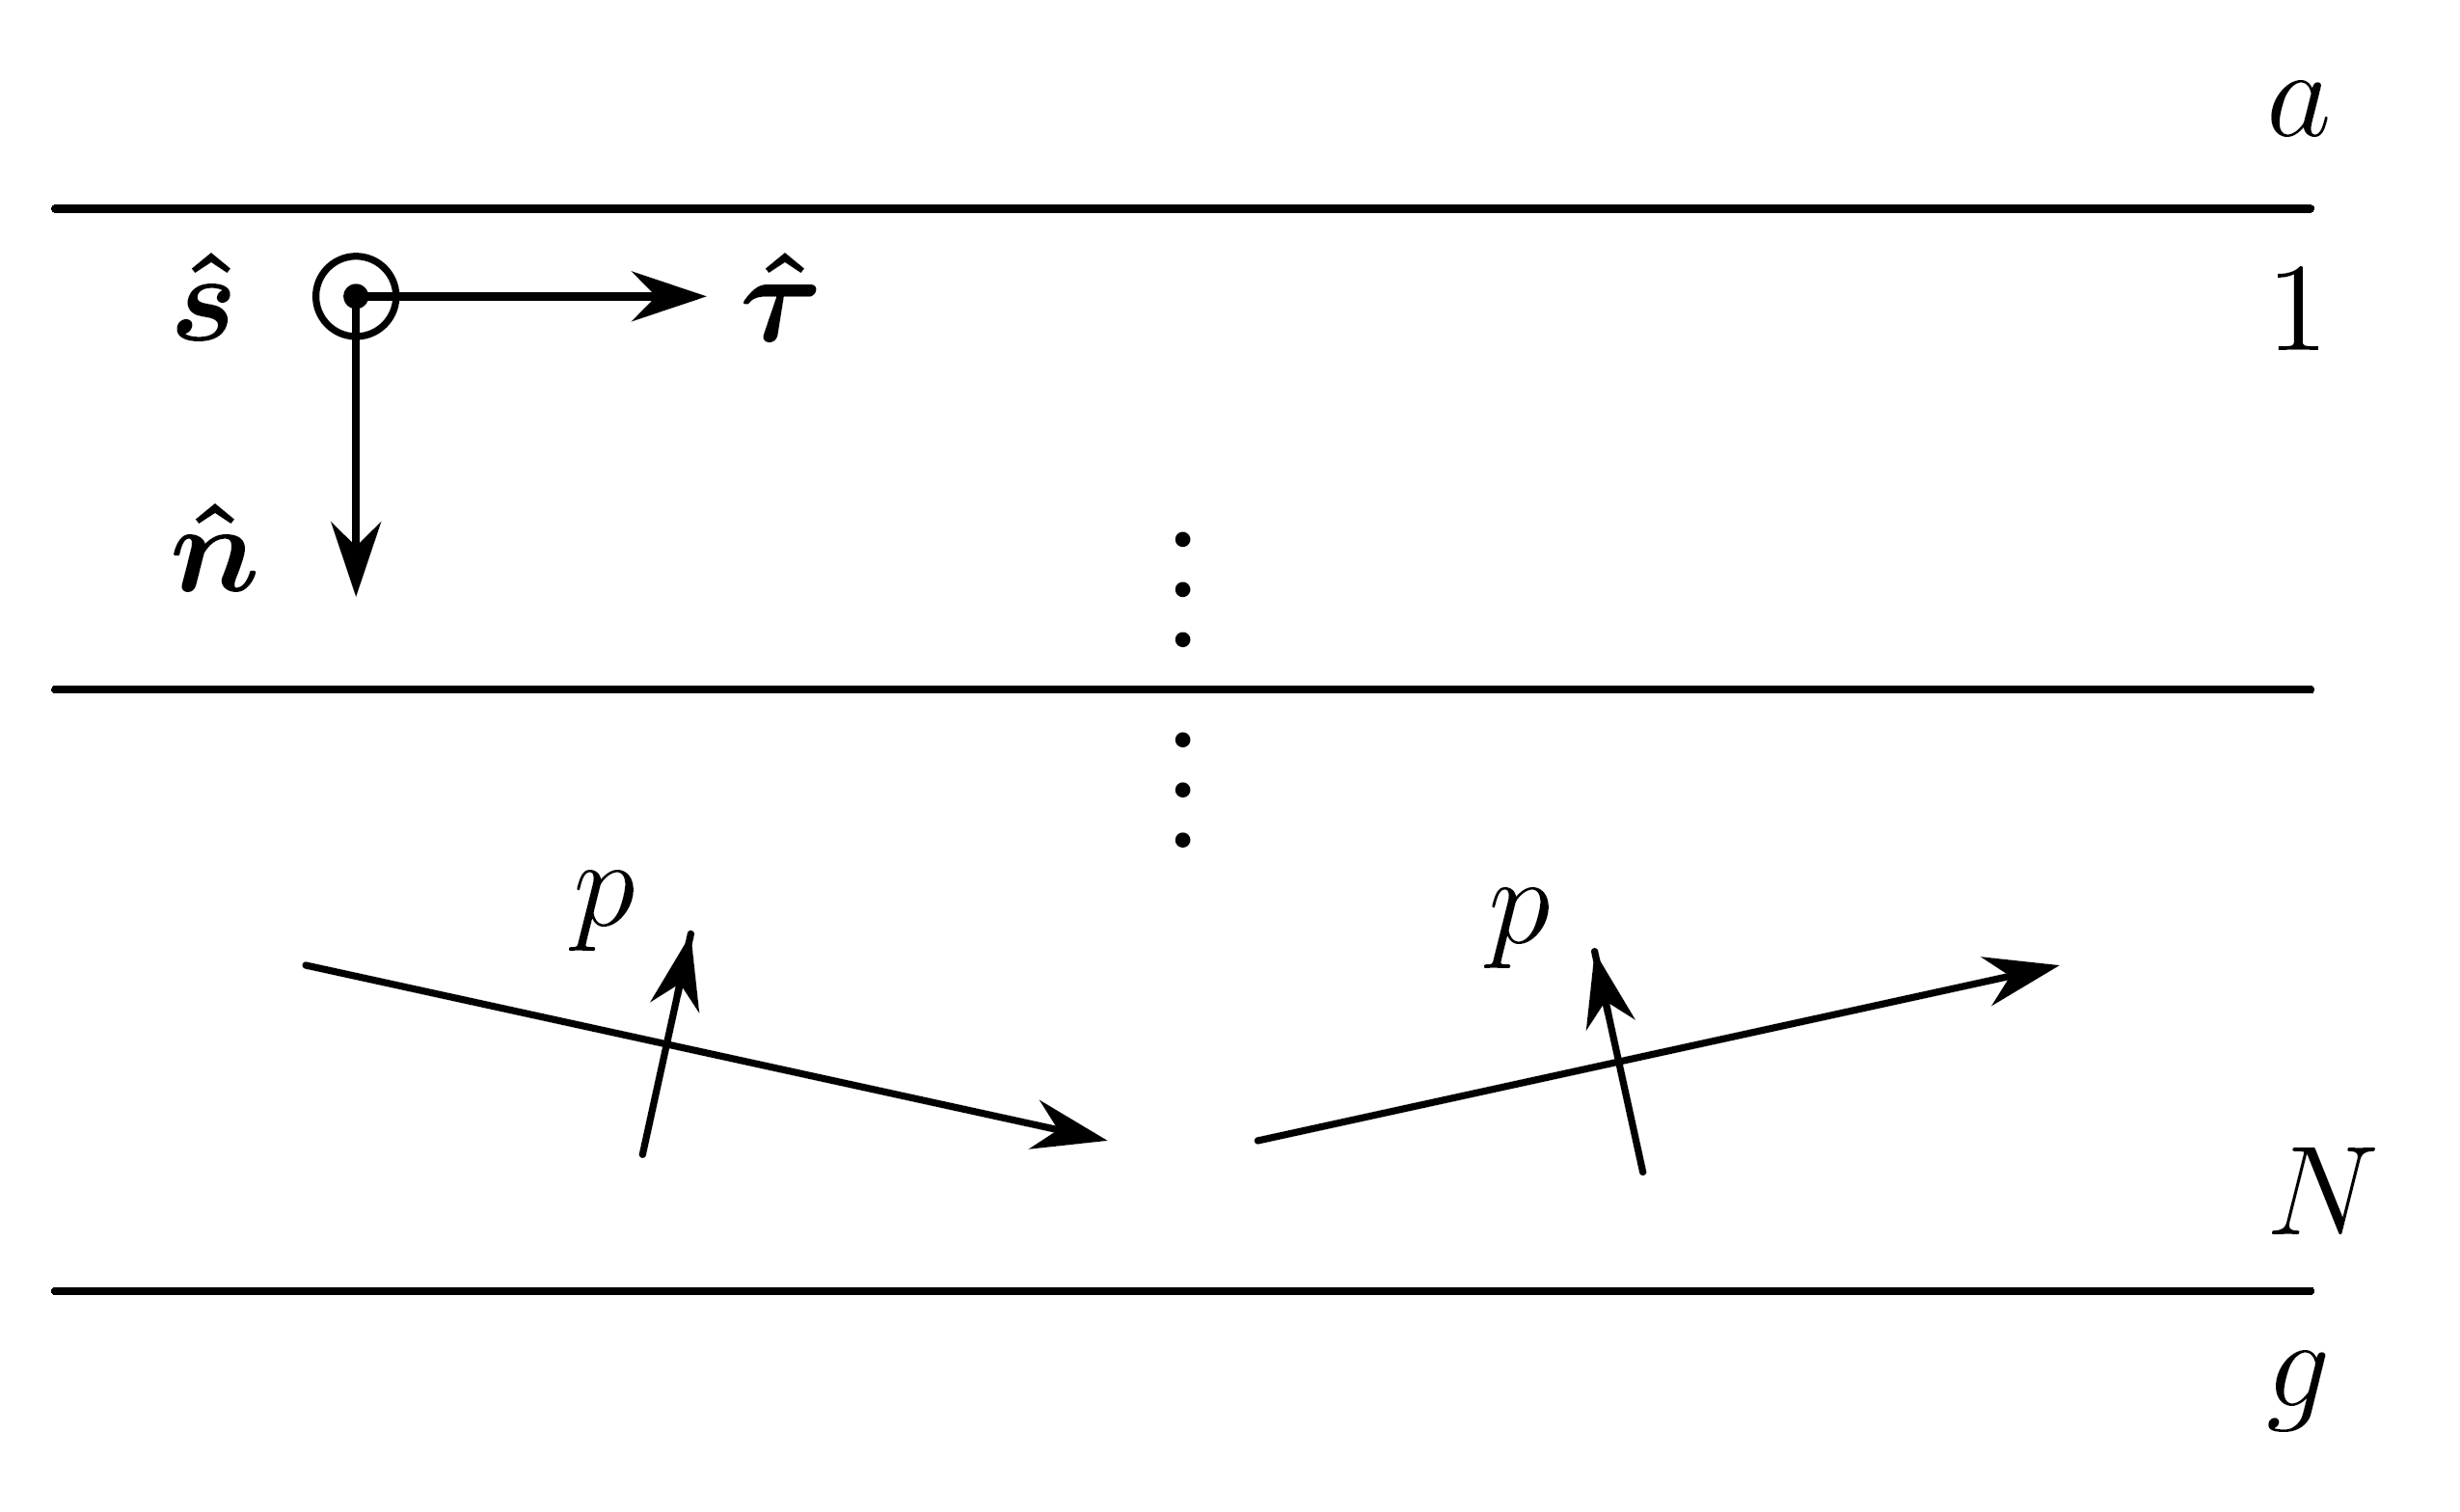
\includegraphics[width=\textwidth]{thin_film_fig/optical_dielectric_film.png}
		\caption{光学介质膜}
		\label{介质膜示意图-光学介质膜}
		\label{光学介质膜}
	\end{subfigure}
	\hfill
	\begin{subfigure}[b]{0.48\textwidth}
		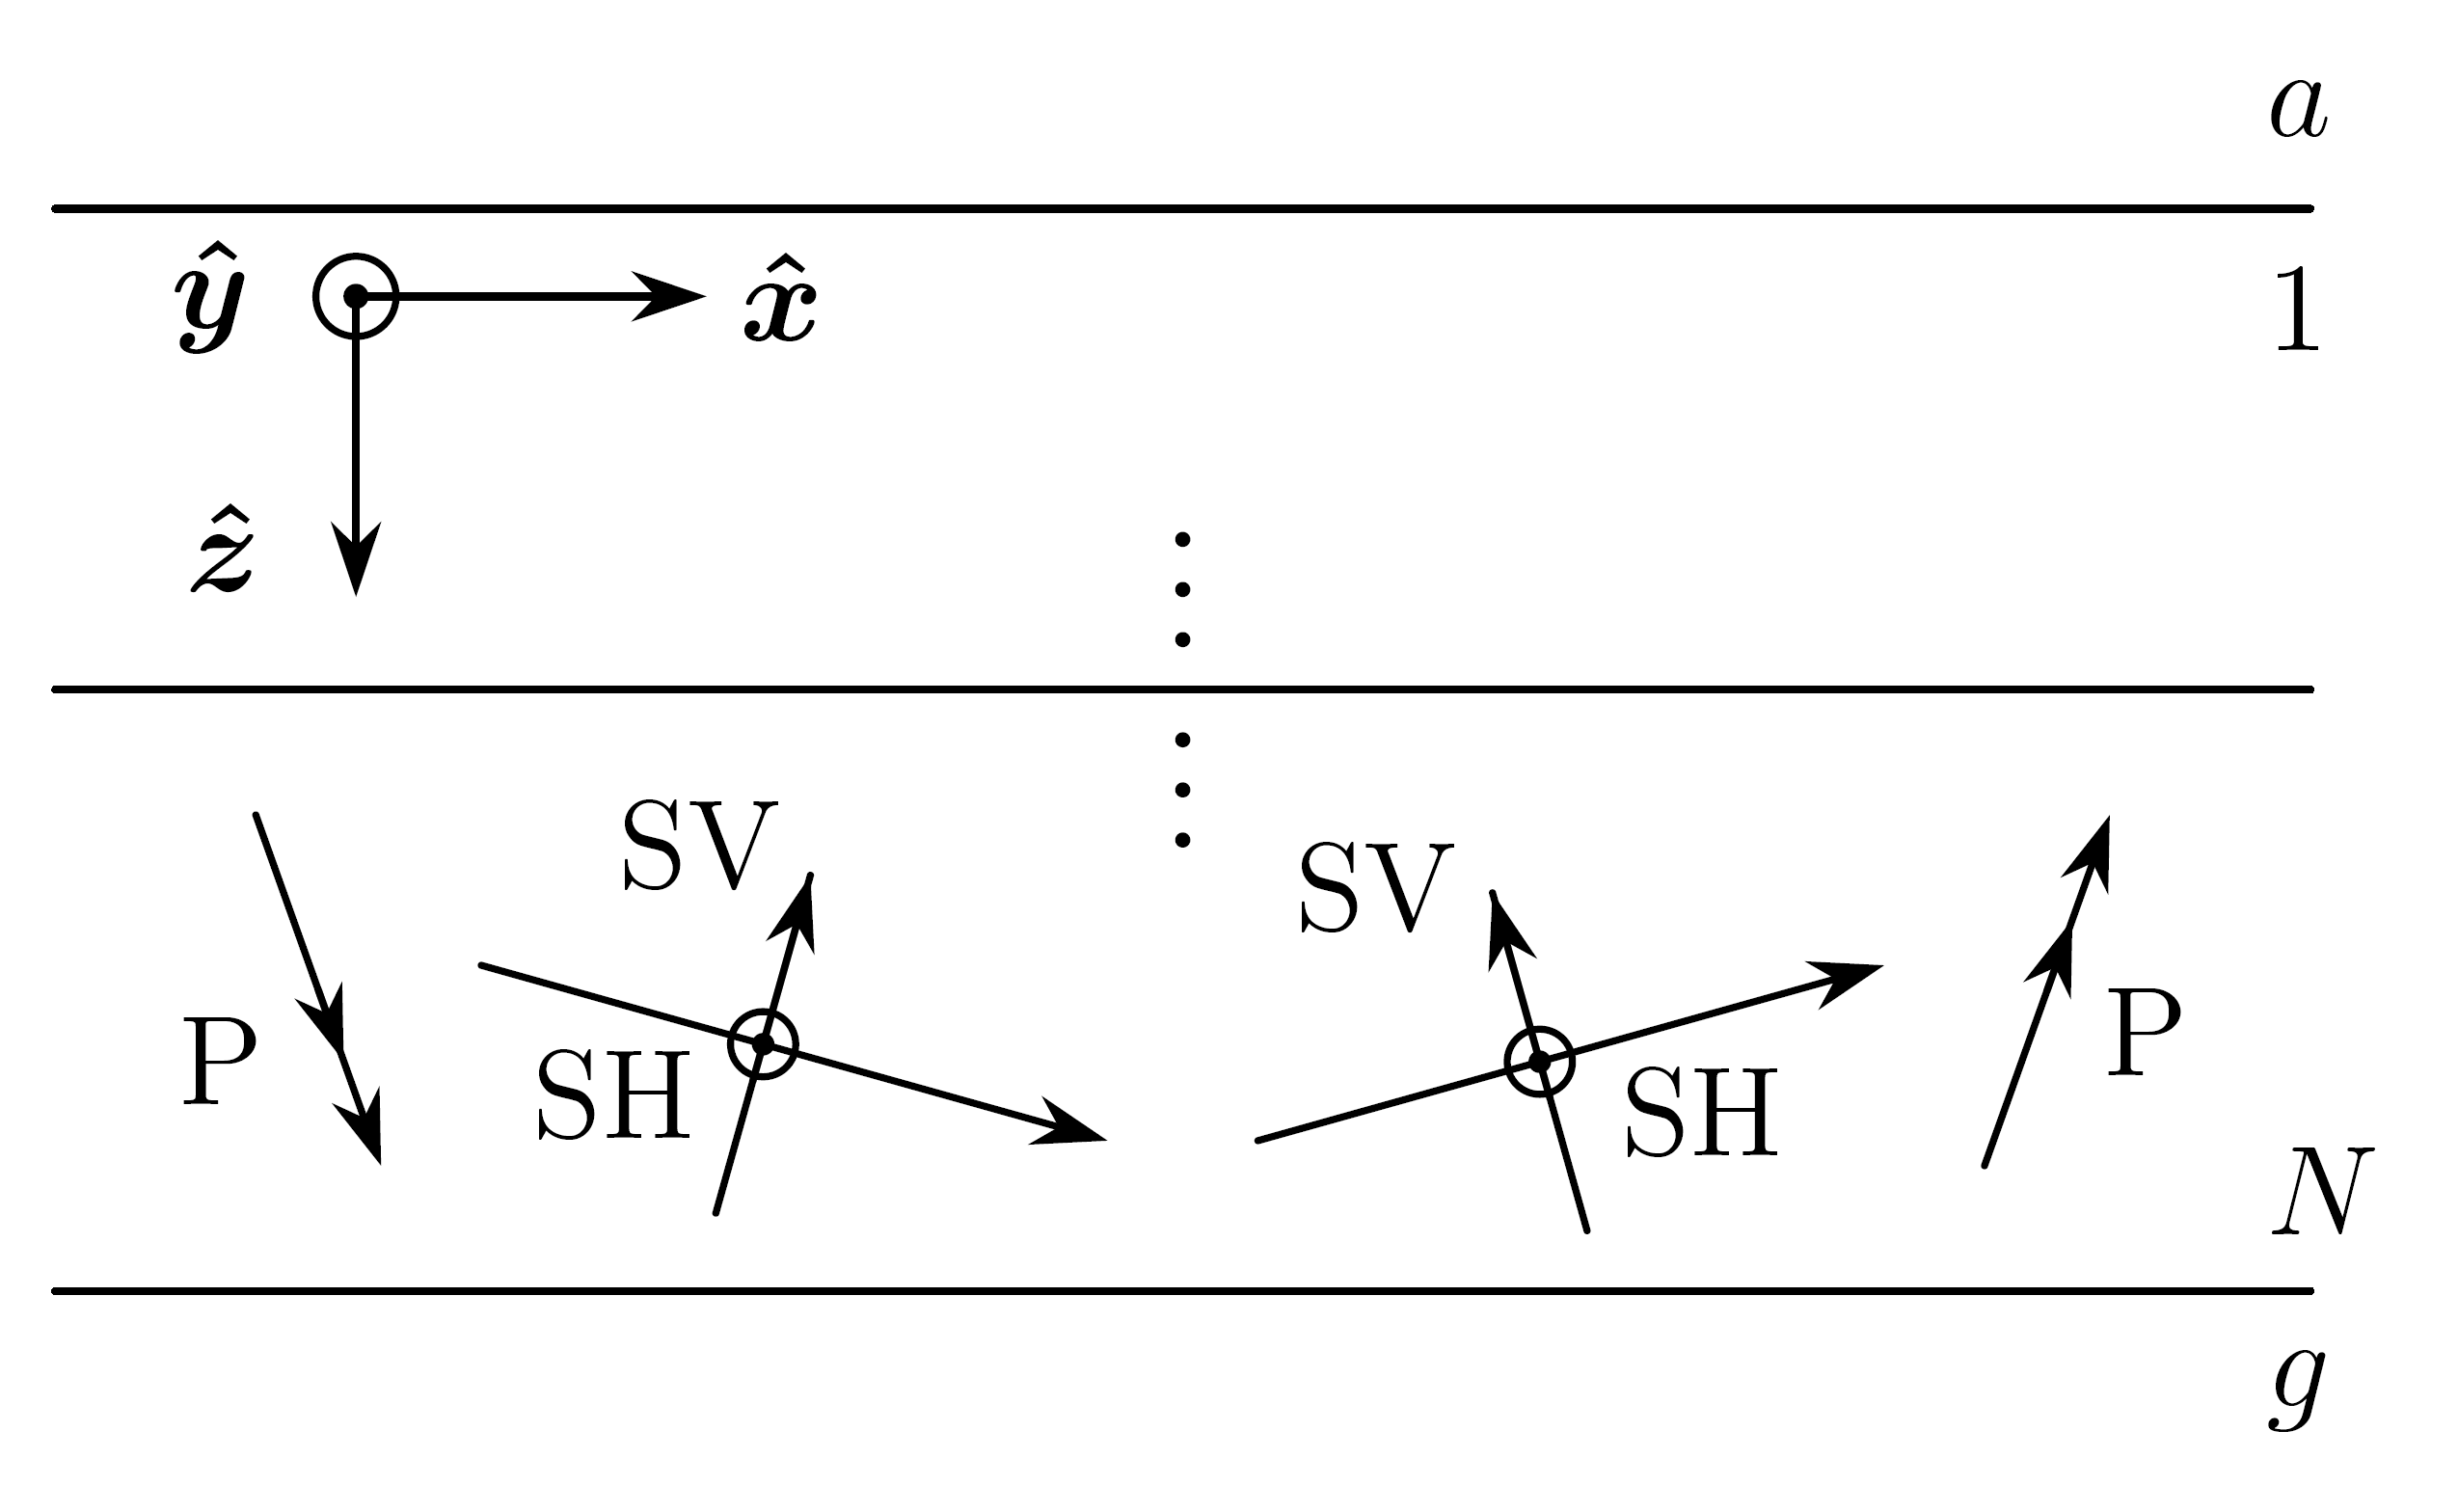
\includegraphics[width=\textwidth]{thin_film_fig/elastic_dielectric_film.png}
		\caption{弹性介质膜}
		\label{介质膜示意图-弹性介质膜}
		\label{弹性介质膜}
	\end{subfigure}
	\caption{介质膜示意图}
	\label{介质膜示意图}
\end{figure}